\chapter{Motivations}
\minitoc%


Dans le cadre de ce stage, les données que l'on traite sont des données du secteur de l'énergie, et plus particulièrement des données de production électrique. On dispose ainsi de plusieurs éoliennes identifiées par le tag "id\_[identifiant de l'éolienne]" dont l'énergie produite est mesurée toutes les demies heures, et ce pendant 4 ans (de de 2014 à 2017).
Cette énergie produite est dénommée la courbe de charge (que l'on abbrégera par \textbf{CDC} par la suite). Il est cependant plus utile de s'intéresser au facteur de charge (ou \textbf{FDC}) qui est défini comme

\begin{equation*}
\displaystyle\textsf{Facteur de Charge} = \frac{\textsf{Courbe de Charge}}{\textsf{Puissance Installée}}
\end{equation*}

On en déduit que \textbf{FDC} doit nécessairement être compris entre 0 et 1. C'est entre autre aussi une manière de détecter des anomalies et données atypiques comme la surproduction d'énergie par rapport à ce qui était attendu de la part d'un parc éolien ou encore un défaut de capteur (tension / intensité, ...) qui mesure la courbe de charge. Voici notamment l'exemple de données éoliennes :


\begin{center}
	période : Première semaine de Juin 2015
	
	\scalebox{1}{
		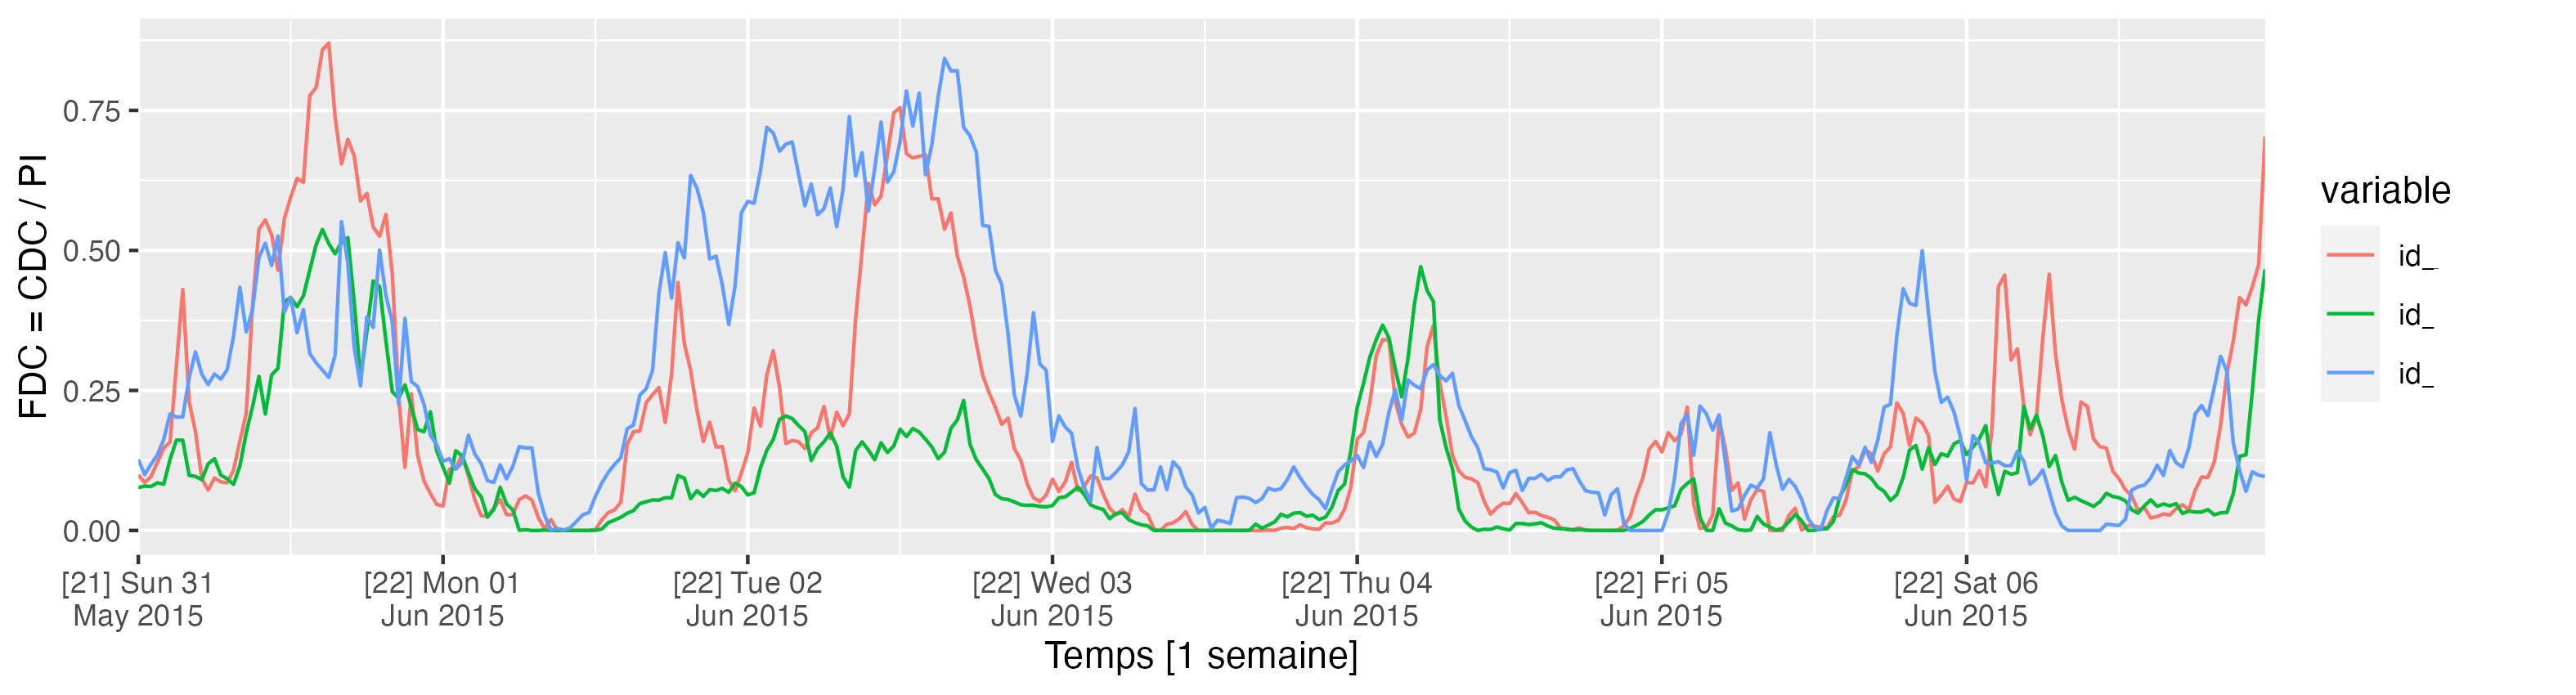
\includegraphics[width=0.85\textwidth]{Images/motivation/test__slice_graph__2015__id_1_2_3__week_1.jpg}
	}
\end{center}

\begin{figure}[H]
	\centering

	période : Juillet 2015

	\scalebox{1}{
		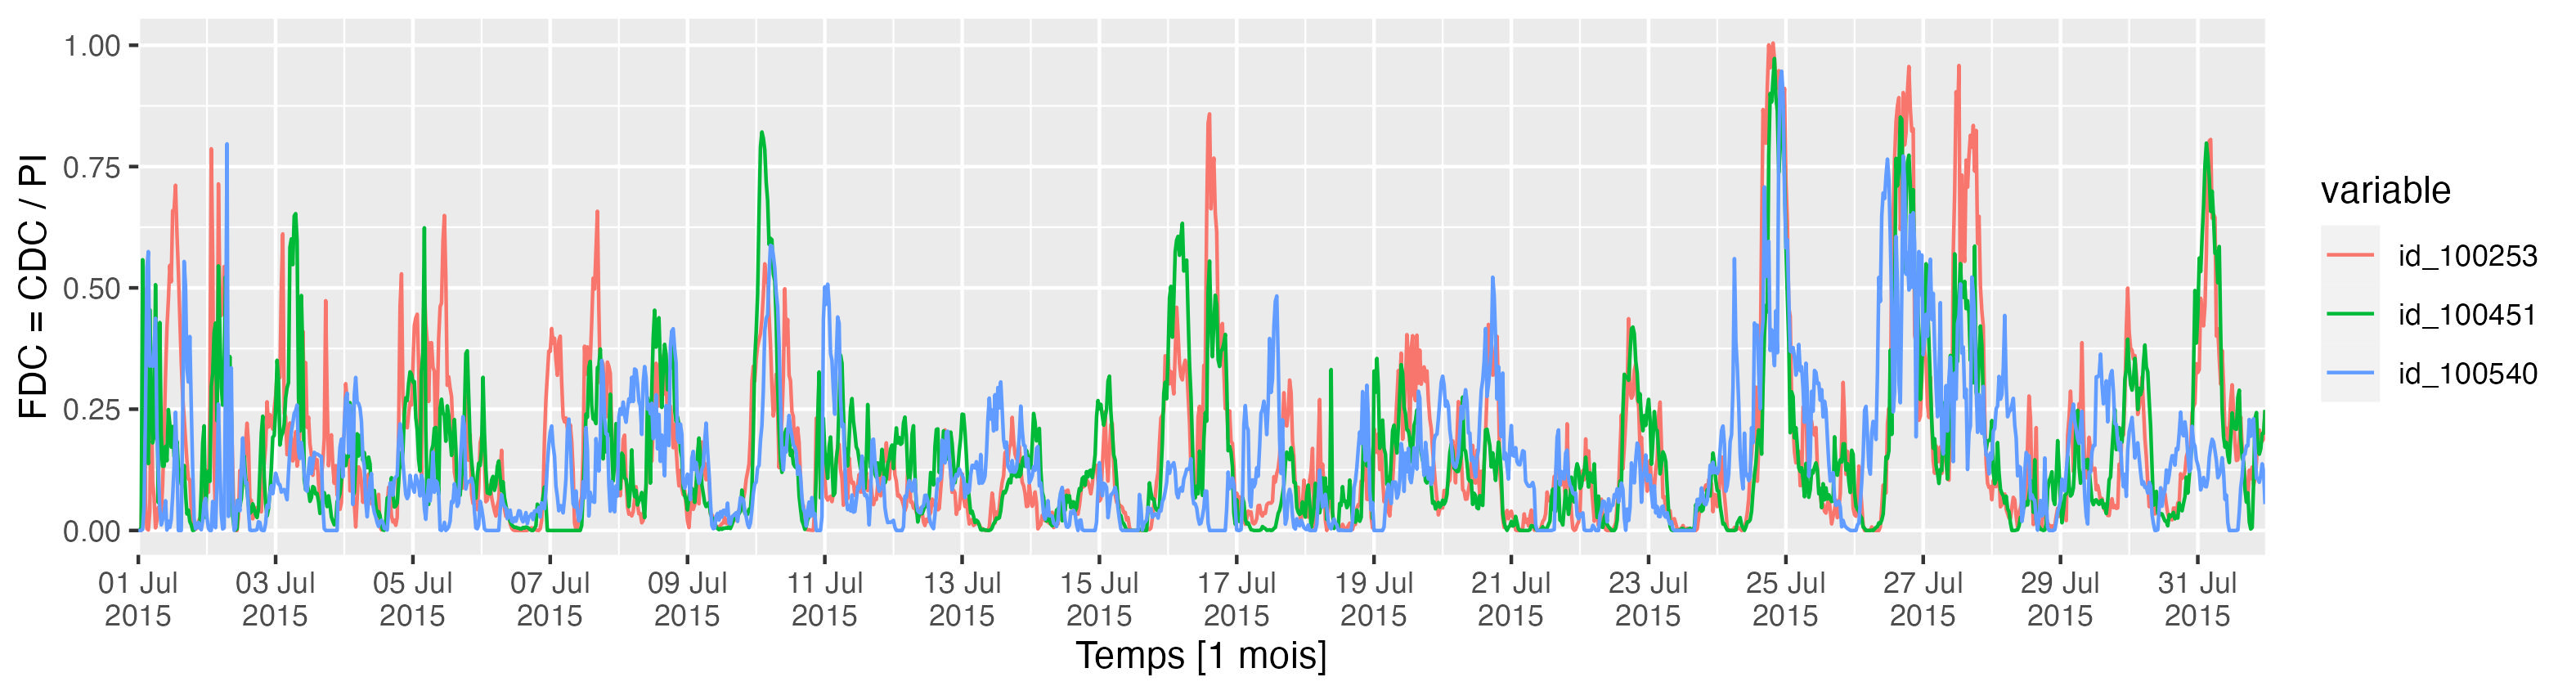
\includegraphics[width=0.85\textwidth]{Images/motivation/test__slice_graph__2015_07__id_1_2_3.jpg}
	}
	\caption{Courbes de charges éoliennes sur 3 premiers parcs éoliens}
	\label{fig:courbes_de_charge}
\end{figure}

\bigskip

Les données qui sont traitées dans le cadre de ce stage sont, entre autres, des courbes de charge observées chaque demie-heure de production électrique éolienne ou photovoltaïque. Le schéma d’observation est donc le \og common-design \fg. C'est-à-dire que les temps d'observations sont ici déterministes à intervalle de temps fixe.

\smallskip

Bien que la différenciation en analyse de séries temporelles soit une méthode efficace pour éliminer la tendance, qu'elle soit saisonnière ou non, permettant ainsi une bonne analyse des données; ces modèles présentent des limites en termes de prédiction à long terme, les rendant moins utiles lorsque l'objectif est de prédire à moyen ou long terme. De plus, ces modèles, ainsi que différents modèles de machine learning populaires, estiment les données courbe par courbe ce qui ne tire pas profit du fait que les observations aient une forme similaire entre les courbes.

\smallskip

Une première idée serait d'utiliser un modèle de série temporelle ARIMA afin de modéliser la dynamique des courbes de charge.


% \book{ \textbf{Un peu d'histoire sur les séries temporelles \ldots}        
\info{une grande partie des informations présentées dans cette section histoire provient de la référience ~\cite{time_series_brief_history} }


\smallskip

Parmi les étapes importantes du développement des séries temporelles, on peut noter l'article \emph{Time Series Analysis : Forecasting and Control} de Box et Jenkins (1970) qui introduit le modèle ARIMA et une approche aujourd'hui standarde d'évaluation du modèle à utiliser ainsi que son estimation. Ce développement est dû en grande partie à l'utilisation de telles données dans les secteurs économiques et des affaires afin de suivre l'évolution et la dynamique de différentes métriques

\smallskip

L'étude des séries temporelle a été divisée en l'étude du domaine fréquentiel, qui étudie le spectre des processus pour le décomposer en signaux principaux, et du domaine temporel, qui étudie les dépendances des indices temporels. L'utilisation de chacune des approches était sujet à débats mouvementés jusqu'aux alentours de l'an $2000$.

\smallskip

Le développement des capacités de calcul a été une révolution notamment pour l'identification des modèles (le critère AIC, l'estimation par vraissemblance dans les années $1980$, \ldots).
% modèles à espace d'états et le filtre de Kalman pour évaluer cette vraissemblance efficacement, MCMC, \ldots).

\smallskip

À partir des années $1980$, les modèles non linéaires émergent (ARCH par Engle, modèles à seuil \ldots) et trouvent application en économie notamment. Enfin l'étude multivariée (modèle VAR) fait surface dans les années 1980 par Christopher Sims~\cite[ \href{https://pubs.aeaweb.org/doi/pdf/10.1257/jep.15.4.101}{lien de l'article} ]{VAR_paper}

\smallskip

Une large partie de la théorie s'appuie notamment sur l'étude des racines de l'unité, en considérant un polynôme d'opérateur $P(B) = (I + \sum_k a_k B^k)$ à partir duquel les relations d'autocorrélations peuvent se ré-écrire.
% }


Toutefois, l'utilisation d'un modèle ARIMA ne permet de modéliser la dynamique du phénomène étudié. En effet, la sélection d'un modèle ARIMA sur le critère du BIC sélectionnait, peu importe le parc éolien, un modèle auto-régressif d'ordre 0. Ainsi le modèle sélectionné considérait les irrégularités de la courbe de charge, dont on attend que le processus duquel elle est issue soit très irrégulier (de par sa complexité), comme étant du bruit. On en conclut que ces modèles peuvent ne pas capturer efficacement la structure complexe des données.

\bigskip

\noindent
\fbox{%
  \parbox{\textwidth}{
    Afin de prédire sur le long terme, nous allons donc adopter une approche basée sur les données fonctionnelles pour capturer la structure de la consommation. Cette approche permettra de d'exploiter une information clé : la similarité entre les courbes observées. 
    }%
}

\question{
	\centering
	\smallskip

	Qu'est-ce qu'une donnée fonctionnelle ?
}

Une donnée est dite fonctionnelle lorsque la variable aléatoire qui nous intéresse n'est plus une variable aléatoire à valeur dans $\mathds R^d$, comme le statisticien a l'habitude de manipuler, mais une variable aléatoire à valeur dans un espace de fonction. Concrètement, chaque réalisation n'est plus un nombre mais bien une courbe toute entière indexée (le plus souvent) sur un intervalle $\mathcal T$.

\begin{figure}[H]
	\centering
	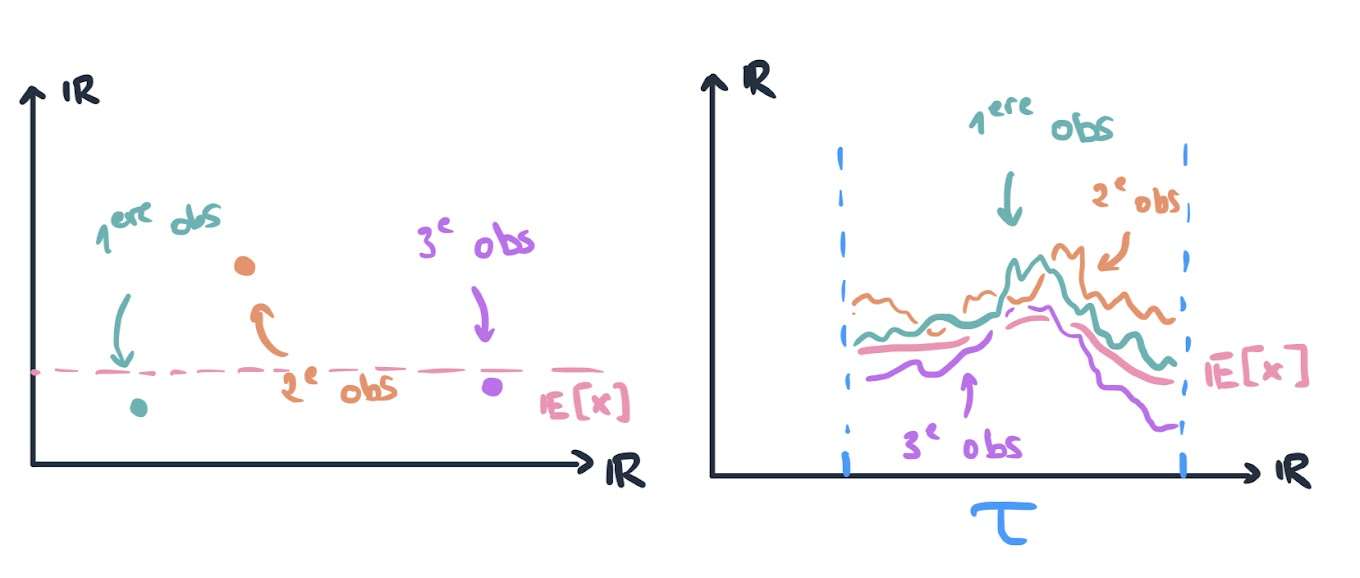
\includegraphics[width=0.85\textwidth]{Images/motivation/donneesRvsFD.jpg}
	\caption{Différence entre donnée fonctionnelle et donnée réelle}
	\label{img:RvsFD}
\end{figure}

Si le statisticien est déjà à l'aise avec l'idée qu'une variable aléatoire réelle identiquement distribuéé puisse modéliser une expérience répétable provenant d'un même phénomène, il pourra se convaincre que les données fonctionnelles permettent elles aussi de modéliser des expériences en lien (fonctionnel) avec un certain paramètre. Et c'est le lien entre les deux valeurs, cette fois-ci, qui provient d'un même phénomène.

\bigskip

Donnons en un exemple : observons la consommation électrique d'un foyer dans une journée. Lorsque l'on travaille sur $\mathds R$, on s'intéresse à sa consommation électrique disons en l'instant $t = 12\mathsf{h}$. Formellement :

\begin{equation*}
	\mathcal T \, \isdef [\, 0,24 \,[ \quad = \textsf{1 jour avec } t \textsf{ en heure}
\end{equation*}

La consommation du foyer $i$ à midi, notée $y_i$, suit la loi d'un phénomène général $Y$, comme une loi normale $\mathcal N\left( 0.27 \, \, kW\mathsf h, 0.1^2 \right)$
%
\footnote{ ordre de grandeur de la consommation électrique d'un foyer en France calculé à partir des données d'ENGIE disponibles librement ~\cite{engie-data-conso-moy-par-an}. \textbf{La variance est arbitraire}, tout comme le choix de la loi juste afin de servir d'exemple. }
%
par exemple. Travailler sur des données fonctionnelles dans ce cadre c'est étudier non plus la consommation $y_i$ à midi, mais regarder l'ensemble de sa consommation en même temps sur toute la journée $y_i(t) = x_i(t)$ avec $t \in \mathcal T$.

\bigskip

On remarque ainsi que toutes les consommations électriques le long de la journée d'un foyer à l'autre suivent la même tendance : on consomme plus le matin avant le travail et le soir alors que pendant la journée on consomme moins car on est au travail. Ainsi c'est la fonction $x_i : \mathcal T \longrightarrow \mathds R$ qui suit la loi d'un phénomène $X$ général. Ce que l'on vient de dire c'est que la \textbf{relation} entre le temps $t \in \mathcal T$ et la consommation électrique ${\, y_i(t) \,}$ est elle même sujet à une loi plus générale. Grossièrement, les courbes auront la même allure, mais chaque individu a sa consommation propre.

\bigskip

\noindent
Plus formellement : comme on a défini une variable aléatoire réelle comme une application :

\begin{equation*}
	\begin{array}{ccc}\Omega &\longrightarrow& \mathds R\\ \omega &\longmapsto& x = X(\omega)\end{array}
\end{equation*}

\noindent
On définit de même une donnée fonctionnelle comme une application :

\begin{equation*}
	\begin{array}{ccc}\Omega &\longrightarrow& \colorize{\mathcal C^0(\mathcal T, \mathds R)}\\ \omega &\longmapsto& x = X(\omega)\end{array}
\end{equation*}

\noindent
Ce que l'on observe sont donc les valeurs des paramètres $t \in \mathcal T$ ainsi que l'image de $t$ par $x$ : $y = x(t)$. Les points que le statisticien observe sont donc les couples de la forme $(t_k^{(\textsf{individu } i)}, y_k^{(\textsf{individu } i)})_{i\in \llbracket 1, m \rrbracket}$, générés par le processus aléatoire $X$ dont la réalisation est la véritable courbe $x_i$ de l'individu $i$ que l'on souhaite estimer pour travailler avec.

\bigskip

\noindent
\info{Il existe différentes façons de définir les données fonctionnelles, une définition possible est la suivante:

	\begin{equation*}
		\begin{array}{ccc}\Omega \times \mathcal T &\longrightarrow& \mathds R \\ ( \omega , t ) &\longmapsto& X(\omega , t) = y\end{array}
	\end{equation*}


	Cependant, cette représentation ne permet pas une interprétation clé en main du concept mais est certainement plus commode à manipuler pour les mathématiciens dans certains contextes. Cette approche est un point de vue de type "processus stochastique" et diffère du point de vue "élément aléatoire" comme traité de façon claire dans ~\cite{HsingEubankTheoreticalFoundationsOfFDA}.
}

\pagebreak

% \book{ \textbf{\ldots et un peu d'histoire sur les données fonctionnelles}
\info{Pour une description plus complète de l'histoire du développement de l'analyse fonctionnelle, on pourra se référer à \href{https://anson.ucdavis.edu/~mueller/fdarev1.pdf}{\textcolor{flatuicolors_blue_deep}{cet article de Wang, Chiou et Müller}}~\cite{wang2016functional}}


Bien que l'histoire du développement de l'Analyse de Données Fonctionnelles (FDA) puisse être retracée jusqu'aux travaux de Grenander et Karhunen~\cite{karhunen1946spektraltheorie} dans les années 1940 et 1950, où l'outil a été utilisé pour étudier les courbes de croissance en biométrie, ce sous-domaine de la statistique a été étudié de manière systématique à partir des années 1980.

\bigskip

En effet, c'est J.O. Ramsay qui a introduit l'appellation de "données fonctionnelles" en 1982~\cite{ramsay1982data} et qui contribuera en partie à sa popularisation. La thèse de Dauxois et Pousse en 1976 sur l'analyse factorielle dans le cadre des données fonctionnelles\cite{dauxois1976analyses} a ouvert la voie à l'analyse par composante principale fonctionnelle (FPCA), un outil clé pour l'étude des données fonctionnelles. La FPCA permet d'étudier des objets fonctionnels qui sont de dimension infinie, difficiles à manipuler et impossibles à observer empiriquement, en dimension finie et surtout sur $\R d$ que l'on connait bien.

\bigskip

Au cours des années 2000, de nombreux outils statistiques déjà développés pour des données à valeurs dans $\R d$ depuis un siècle, tels que la régression linéaire (éventuellement généralisée), les séries temporelles ou encore les modèles additifs, ont été adaptés aux données fonctionnelles.
Par exemple, les modèles de régression linéaire fonctionnelle ont été développés avec une réponse fonctionnelle~\cite{ramsay1991some} ou scalaire~\cite{cardot1999functional} en 1999.
Les modèles linéaires généralisés ont également été étudiés~\cite{james2002generalized,muller2005generalized}, avec l'estimation de la fonction de lien par méthode non paramétrique à direction révélatrice \emph{(Single Index Model)} récemment étudiée en 2011~\cite{chen2011single}.
Cette méthode avait déjà été utilisée en économétrie pour des données de $\R d$ depuis 1963~\cite{sharpe1963simplified}, et leur estimation directe a été étudiée une décennie auparavant par M.Hristache, Juditsky et Spokoiny~\cite{hristache2001direct}. De même, les modèles additifs ont été étendus aux données fonctionnelles en 1999 par Lin et Zhang~\cite{lin1999inference}.
Enfin, le livre de Bosq, \emph{\textcolor{flatuicolors_blue_devil}{Linear Processes in Function Spaces : Theory and Applications}}~\cite{bosq2000linear}, publié en 2000, a contribué au développement des séries temporelles pour les données fonctionnelles.

\bigskip

Depuis lors, des ressources telles que l'ouvrage de Kokoszka et Reimherr, \emph{\textcolor{flatuicolors_blue_devil}{Introduction to Functional Data Analysis (2017)}}~\cite{kokoszka2017introduction}, rendent la théorie et la mise en production des méthodes d'analyse et de prédiction de données fonctionnelles plus accessibles.
% }


\pagebreak


Maintenant que l'on possède une meilleure intuition de ce que sont les données fonctionnelles, il est naturel de se demander pourquoi le choix de modéliser notre phénomène par des données fonctionnelles serait particulièrement judicieux. Pour cela, rappelons nous les difficultés que l'on avait rencontrées dans le cadre de nos données de production électrique en utilisant un modèle de série temporelle classique :

\info{
    \textbf{Rappel : }

    "Ainsi le modèle \colorize{(arima)} sélectionné considérait les irrégularités comme étant du bruit $[\ldots]$ Afin de prédire sur le long terme, nous allons donc adopter une approche basée sur les données fonctionnelles pour capturer la structure de la consommation $[\ldots]$"
}


\question{\smallskip
\centering
    Pourquoi est-ce que l'on s'intéresse autant à la régularité des données que l'on étudie ici ? Et surtout, en quoi est ce que les données fonctionnelles vont nous permettre de mieux capturer la régularité ?
    }

Comme mentionné auparavant, la production électrique est un phénomène très irrégulier [~\ref{fig:courbes_de_charge}] étant influencé par la consommation, la météo, etc. Par conséquent, la prévision de ces courbes de charge doit prendre en compte la nature fondamentalement irrégulière du phénomène afin de proprement le modéliser et, en définitive, mieux le prédire. Ce qui est notamment contraire à la plupart des méthodes qui utilisent des fonctions de classe $\mathcal C^2$ pour lisser les points observés en données fonctionnelles, ce qui limite la prédiction à des courbes de nature $\mathcal C^2$. Cela est d'autant plus critique lorsque l'on cherche à estimer le processus moyen ou l'opérateur de covariance du processus, car ces derniers sont estimés à partir des courbes lissées, qui détruisent toute l'information irrégulière si elle n'est pas prise en compte, impactant significativement l'estimation des objets qui nous intéressent en tant que statisticien.

\editlater{introduire photo qui superpose un mouvement brownien et le lissage spline de ce même mouvement brownien}

Il est ainsi important pour des phénomènes de nature irrégulière de ne pas négliger des précautions lors du lissage afin de ne pas perdre l'information irrégulière. L'idée est donc d'estimer dans un premier temps la régularité de notre processus afin de lisser nos données de manière adaptée pour débruiter et prédire des valeurs non observées tout en préservant les informations irrégulières critiques pour la bonne estimation du processus moyen et de l'opérateur de covariance. L'approche fonctionnelle est clé dans l'estimation de cette régularité, car c'est la \textbf{réplication de courbes} de même nature qui permet in-fine d'\textbf{estimer la régularité} du phénomène.

% ~ ——————————————————————————————————————————————————————————






